\documentclass[a4paper,12pt,openbib]{article}

\usepackage{titling}
\usepackage[margin=0.5in,headsep=0.25in,footskip=0.25in]{geometry}
\usepackage{graphicx}
\usepackage{float}


\newcommand{\subtitle}[1]{
	\posttitle{
		\par\end{center}
		\begin{center}\large#1\end{center}
		\vskip0.5em
	}
}

\newcommand{\datacube}[3]{
\begin{figure}[ht!]
	\centering
	\setlength{\unitlength}{1cm}
	\begin{picture}(10,5)
		\put(0,0){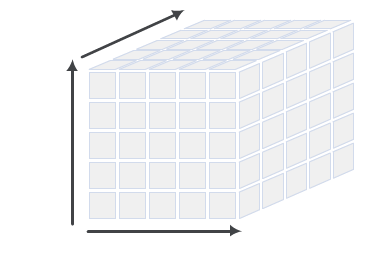
\includegraphics[height=5cm]{cube}}
		\put(1,4.5){#1}
		\put(-0.25,2){#2}
		\put(2,0.0){#3}
	\end{picture}
\end{figure}
}

\newcommand{\drilldown}[1]{
\begin{figure}[ht!]
	\centering
	\setlength{\unitlength}{1cm}
	\begin{picture}(1,1)
		\put(-2,0){
\includegraphics[height=1cm]{drill}}
		\put(-3.5,0.5){#1}
	\end{picture}
\end{figure}
}

\begin{document}

% title page
% TODO: Spruce it up
\title{CITS3401 Data Exploration and Mining\\
Project 1}
\subtitle{Medicare Australia Data Warehouse}
\author{Mitchell Pomery\\
21130887}
\maketitle
\abstract{
This document outlines the design choicies for a data cude created to assist Medicare in giving the best service possible.
The original requirements were incomplete and so assumptions were made where necessary.
}
%\newpage

% document

\section*{Introduction}
\paragraph{}
Medicare Australia wishes to use data from it's previous years to assist in making decisions to improve their services, analyse expenditure and detect individuals who are abusing their system.
Each centre stores information about visits in an Online Transaction Prorocessing (OLTP) database, these are then collated at a state and country wide level.
The patient, doctor, treatment and prescriptions for each visit are stored.
This document outlines the data cube designed facilitate in the decision making processes of Medicare.

\section*{Requirements}
\paragraph{}
% TODO: List Requirements
The authors' interpretation of the requirements are listed below.

\begin{table}[h]
\centering
\begin{tabular}{|l|l|l|}
	\hline
		\textbf{Object} & \textbf{Properties} & \textbf{Restrictions} \\
	\hline
		Location && State or Territory in Australia \\
	\hline
		Centre && 3 Centres in each State/Territory \\
	\hline
		Tests && Only one test will occur per visit. \\
	\hline
		Diseases && Only one disease will be diagnosed per visit maximum. \\
	\hline
		Store & Interior Design & 3 restaurants in each country \\
		& Facility Type & 3 different interior designs \\
		&& Facilities are `dine in', `drive through' and `both' \\
	\hline
\end{tabular}
\caption{Requirements}
\label{tab:requirements}
\end{table}

\subsection*{Assumptions}
\paragraph{}
Assumptions were made where the requirements were incomplete or insufficient, to simplify the schema and keep it managable, and to make the scenario as realistic as possible.
% TODO: Assumptions
\begin{enumerate}
	\item Only a small number of patients, diseases, physicians, hospitals, specialists and pathology clinics exist.
	\item Doctors are irellevant, only the name of the clinic matters.
	\item Patients will always visit a General Physician before seeing a specialist.
	\item The cost of treatment, as well as the person or company who pays for the treatment is irrelevant.
	\item People only visit medical centres in their own state.
\end{enumerate}

\section*{Warehouse Schema}
\paragraph{}
A star schema was designed to make the data cube simpler, and the queries faster than a snowflake schema or fact constellation.
\begin{figure}[ht!]
	\centering
	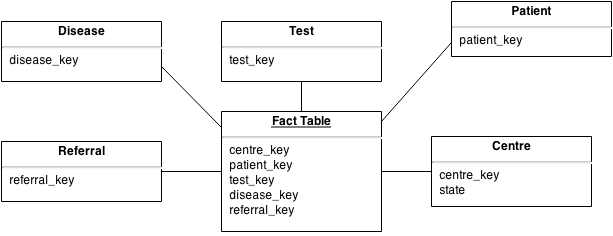
\includegraphics[width=15cm]{schema}
	\caption{Fact Table in Snowflake Schema}
	\label{fig:schema}
\end{figure}

\section*{Prototype Warehouse}
\subsection*{Data Generation}
\paragraph{}
	Prototyape data was generated using the Python script \texttt{gendata.py}.
	It takes sets of words for diseases, clinics, names, medical tests and states, creates random people and outputs information about their visits from 2006 to 2011.
	An attempt has been made to make it reflect reality, by restricting the average persons visits to a couple of times a year, charging based on the location visited and making a small percentage of users abuse the system each year.

\section*{Features}
\paragraph{}
Adds the ability to do...
\begin{enumerate}
	\item expenditure analysis
	\item planning new infrastructure
	\item detecting fraud
	\item policy changes
\end{enumerate}

\subsection*{Expenditure Analysis}
	aa

\section*{Data Cube}
\paragraph{}
	A visualization of the data cube is provided below:
\datacube{Tests}{Time}{Location}
\drilldown{}
\datacube{Tests}{Year}{State}
\drilldown{Drill Down On Year}
\datacube{Tests}{Quarter}{State}
\drilldown{Drill Down On State}
\datacube{Tests}{Quarter}{Clinic}
\drilldown{Drill Down On Tests}
\datacube{Diseases}{Quarter}{Clinic}
\drilldown{Drill Down On Diseases}
\datacube{Specialist}{Quarter}{Clinic}

\end{document}